%!TEX root = ../dokumentation.tex

\chapter{Materialien und Methoden} \label{ch:materialsAndMethods}

% TODO: Linguistische Begriffe (Semantik, Syntax, Pragmatik) erklären

% -   Politikapparat und Parteienlandschaft
% -   Erörterung, welche Medienplattformen und Nachrichtenquellen verwendet werden sollen
% -   Auswahl von Quellen und Sammeln von Daten
% -   NLP-Pipeline
% -   Machine Learning / Clustering

\section{Deutsche Politik in der 19. Legislaturperiode}

\subsection{Bundestagswahl \num{2017}}

\begin{figure}[H]
    \centering
    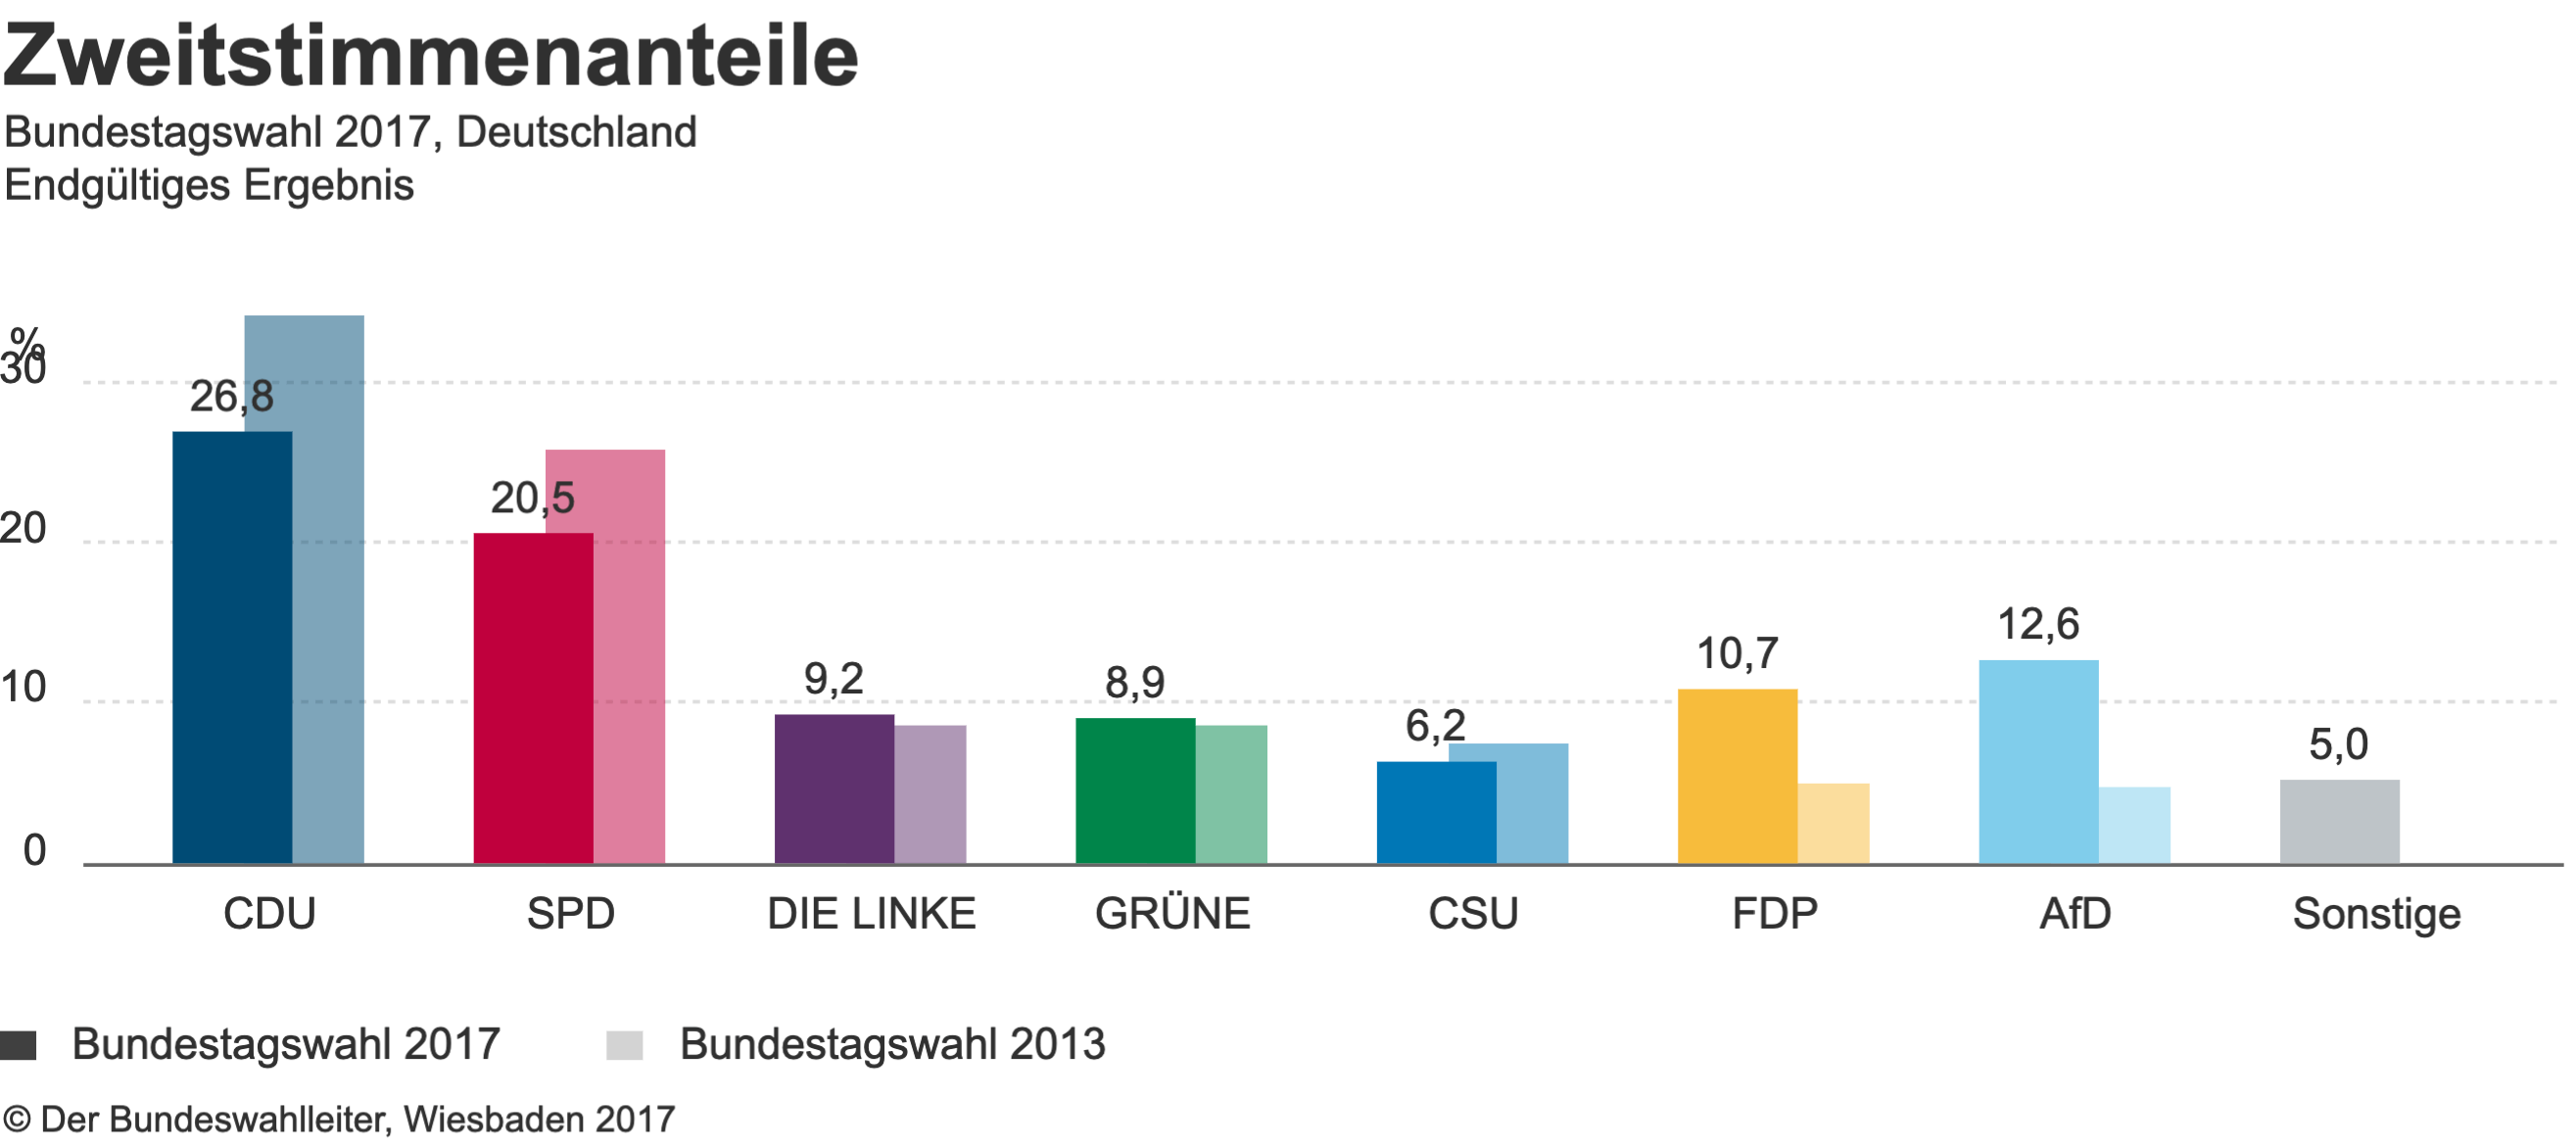
\includegraphics[width=0.9\textwidth]{data/images/ergebnisBtw17.png}
    \caption{Ergebnis der Bundestagswahl \num{2017} \autocite{noauthor_bundestagswahl_nodate}} \label{fig:ergebnisBtw17}
\end{figure}

\citeauthor{schmid_deutscher_2021} \autocite{schmid_deutscher_2021}:
\begin{itemize}
    \item AfD zum ersten Mal vertreten, direkt drittstärkste Kraft
    \item Zum ersten Mal waren sieben Parteien und sechs Fraktionen im Bundestag vertreten → Zeichen für die weiter abnehmende Bindungskraft der alten Volksparteien CDU, CSU und SPD
    \item Union und SPD mit starken Verlusten, SPD verlor dramatisch und fuhr mit \SI{20.5}{\percent} ihr schlechtestes Ergebnis seit \num{1949} ein
    \item FDP Rückkehr ins Parlament
    \item Linke und Grüne leicht verbessert
    \item Jamaika Verhandlungen gescheitert, längste Regierungsbildung aller Zeiten
\end{itemize}

\subsection{Heterogenität der Parteienlandschaft} \label{subsec:heterogenitätParteien}

\citeauthor{niedermayer_entwicklung_2020} \autocite{niedermayer_entwicklung_2020}:
\begin{itemize}
    \item Schrittweiser Verlust an Zustimmung bei Volksparteien
    \item Grüne sind auf dem sich als zweitstärkste Kraft zu etablieren
    \item AfD fest verankert
    \item Wenig Dynamik bei FDP und Linken
    \item Allgemein: Von festem Zweiparteiensystem zu \enquote{einem pluralistischen System an der Grenze zum hochfragmentierten System}
\end{itemize}

\citeauthor{thomeczek_politische_2019} \autocite{thomeczek_politische_2019}:
\begin{itemize}
    \item Zwei Lager: \enquote{links-liberal} und \enquote{rechts-konservativ} / \enquote{bürgerlich}
    \item FDP Sonderrolle: gesellschaftspolitisch liberal, wirtschaftspolitisch rechts
    \item Unterschiedliches Maß an innerer Kohärenz: SPD und CDU weisen insgesamt durchschnittlich weniger hohe Agreement-Index-Werte auf als die anderen Parteien
\end{itemize}

\citeauthor{engler_wettbewerb_2022} \autocite{engler_wettbewerb_2022}:
\begin{itemize}
    \item Viele Alternativen in der Opposition, z.B. Klima (AfD vs Grüne/Linke), Corona (auch FDP gegen zu viele Einschränkungen)
\end{itemize}

\begin{figure}[H]
    \centering
    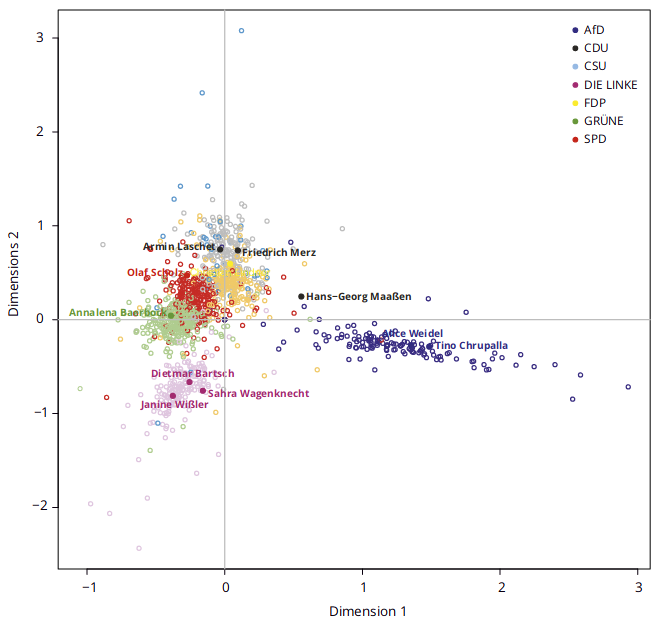
\includegraphics[width=0.5\textwidth]{data/images/positionierung_ausgewaehlter_kandidaten.png}
    \caption[Positionierung ausgewählter Kandidaten \autocite{saltzer_bundestagswahl_2022}]{Positionierung ausgewählter Kandidaten innerhalb eines zweidimensionalen politischen Raums \autocite{saltzer_bundestagswahl_2022}} \label{fig:positionierungAusgewaehlterKanidaten}
\end{figure}

\subsection{Besondere Ereignisse im Untersuchungszeitraum}

% TODO: Weitere durchgeführte Wahlen ansprechen

\citeauthor{schmid_deutscher_2021} \autocite{schmid_deutscher_2021}:
\begin{itemize}
    \item Corona
    \item Ende Einsatz der Bundeswehr in Afghanistan, Machtübernahme der Taliban
    \item Flut in Teilen von NRW / RLP
\end{itemize}

\subsection{Themenschwerpunkte}

\begin{figure}[H]
    \centering
    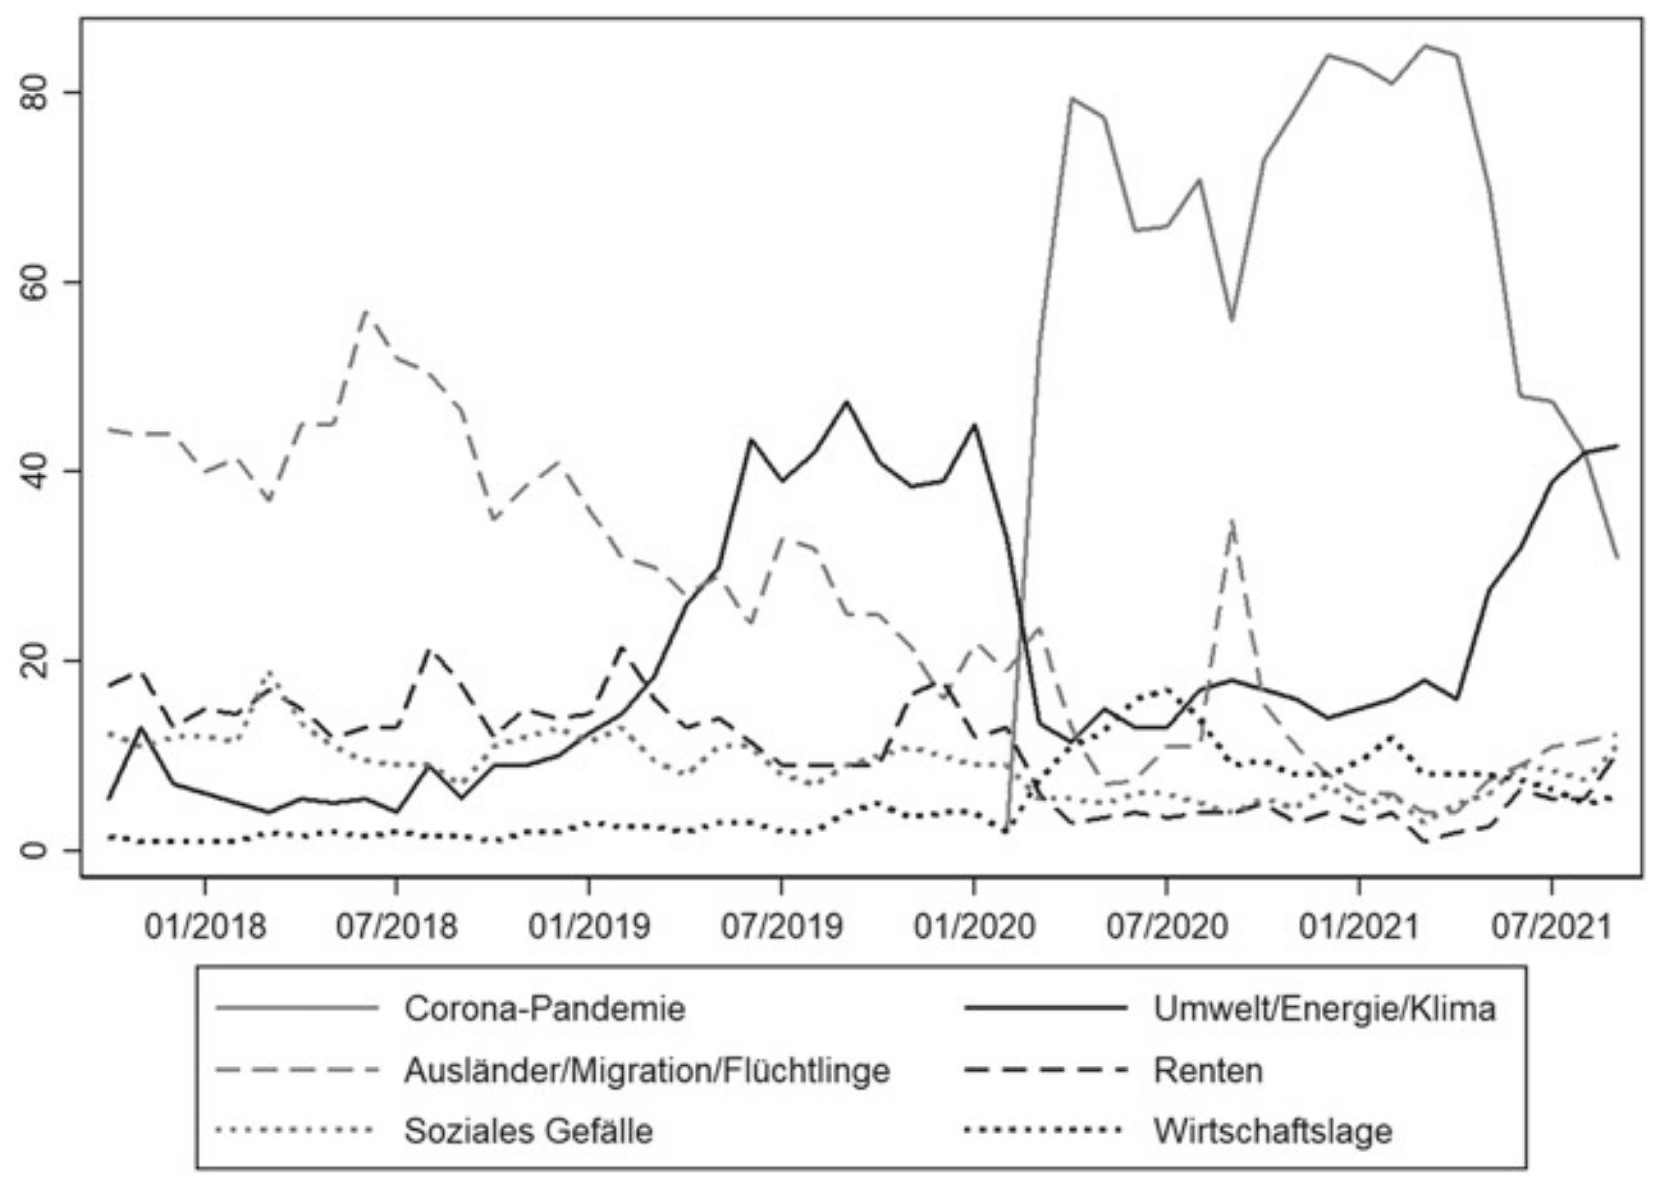
\includegraphics[width=0.8\textwidth]{data/images/themenkonjunktur.png}
    \caption{Verlauf der wichtigsten politischen Themen während der 19. Wahlperiode \autocite{engler_wettbewerb_2022, forschungsgruppe_wahlen_forschungsgruppe_nodate}} \label{fig:themenkonjunktur}
\end{figure}

\citeauthor{engler_wettbewerb_2022} \autocite{engler_wettbewerb_2022}:
\begin{itemize}
    \item Ab \num{2019} Klimaschutz immer wichtiger, zeitweise wichtigstes Thema
    \item Nach Flutkatastrophe wieder deutlich wichtiger
    \item Corona deutlich am wichtigsten während Pandemie-Zeit
    \item Migration am Anfang sehr wichtig, aber immer weiter abgenommen
    \item Wirtschafts- und sozialpolitische Themen eher im Hintergrund
\end{itemize}

\citeauthor{niedermayer_entwicklung_2020} \autocite{niedermayer_entwicklung_2020}:
\begin{itemize}
    \item Flüchtlingskrise
    \item Klimawandel und Energiewende (Hambacher Forst, Dieselskandal, Hitzewelle Sommer \num{2018}, Popularität von \enquote{Fridays for Future})
\end{itemize}

\section{Feature Engineering}

% TODO: Explain sentiment model and accuracy

\section{Repräsentationsformen von Text}

% TODO: Either describe specific models or the underlying architecture (e.g. fasttext or n-gram method)

Die Theorie hinter Worteinbettungen (engl. Word Embeddings) wurde erstmals anhand von Wörtern, die in einem ähnlichen Kontext auftreten, festgestellt, da diese häufig auch eine ähnliche Bedeutung besitzen (z. B. Augenarzt und Optiker) \autocite[103]{jurafsky_speech_2023}.

Nach \textcite[103]{jurafsky_speech_2023} unterscheiden sich Embeddings in statische und kontextbasierte Word Embeddings.

Herkömmliche Methoden wie \ac{BoW} und \ac{TF-IDF} generieren unkomprimierte Vektoren und skalieren linear mit der Anzahl an einzigartigen Wörtern. Ein alternativer Ansatz dazu sind sogenannte Word Embeddings. Mittels dieser werden Wörter nicht mehr eins zu eins in einzelne Features encodiert, sondern mittels mehrdimensionalen Vektoren\footnote{Häufig bestehen Word Embeddings aus \num{300} Dimensionen} repräsentiert.

\subsection*{\acl{BoW}}

% TODO: Check if formula is correct

\begin{itemize}
    \item \ac{BoW} führt zu Matrizen mit den Maßen \(n(\{v_i\}_{i\epsilon\{1,\dots,n\}}) \times n(rows)\) (Anzahl an einzigartigen Wörtern x Anzahl an Einträgen)
\end{itemize}

\subsection*{\acl{TF-IDF}}

% TODO: Add function for dimensions

\subsection*{FastText}

Lorem Ipsum

\subsection*{GloVe}

% TODO: Check if Spacy uses GloVe or not

Lorem Ipsum

\subsection*{ELMo}

Lorem Ipsum

\section{\acl{ML} Verfahren}

\ac{ML}

% TODO: Add and descripe models used for modeling

\subsection*{BERT}

Lorem Ipsum

\subsection*{LSTM}

Lorem Ipsum

\section{Methodik zur Auswahl}

% Anzahl
% vorhandenes Mapping
% Datenschutz (Tweets)
% Qualität



\section{Zusammenfassung}
